% ===== RUBRIC OF TEACHER'S JOB ASPECTS =====

% A single rubric criterion
\newcommand{\rubriccriterion}[4]{
\stepcounter{rubricquestion}
\section*{\therubricquestion: #1}

\smallskip
\note{Unaware:} #2

\note{Beginner:} #3

\note{Guru:} #4

\medskip
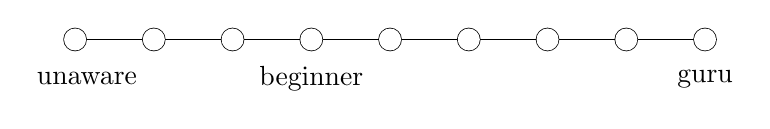
\begin{tikzpicture}
\draw (0,0) -- (8,0);
\foreach \i in {0,1,...,8} % numbers on line
{
\fill[black] (\i,0) circle (1.5 mm);
\fill[white] (\i,0) circle (1.4 mm);
}
\node at (0.15, -0.5) {unaware};
\node at (3, -0.5)    {beginner};
\node at (8, -0.5)    {guru};
\end{tikzpicture}
}

\restoregeometry
\chapter*{Rubric for teaching skills}
\label{rubric}

The following pages present a scoring rubric for teaching skills. Many teachers (young and old alike) don't perceive all the different levels and dimensions of the teaching skill. This is often caused by them not seeing these skills in others. After months or years of teaching, there may come a moment when you realize that the space for improvement is much larger than you expected\punct{.}\footnote{More information can be found for example in the book \emph{How Learning Works: Seven Research-Based Principles for Smart Teaching}.}

\section*{What is a scoring rubric?}

A scoring rubric is a self-assessment tool (helping you see and describe your skills and knowledge).
Firstly, it helps you to perceive and name all the fundamental parts of a concept (e.g., being able to program means being able to design an algorithm, work with memory effectively, know the syntax). Secondly, it enables you to evaluate your competence in these parts (e.g., I'm able to design a working algorithm, though I find it problematic to express it in code and I don't optimize memory usage at all).

\section*{How to use the rubric for teaching skills?}

Fill in the rubric at the beginning of the semester (indicate the level of your skill on the scale). Choose 1--3 areas you to focus on this semester. If you want to be thorough, try to think of specific actions to do and useful indicators of your progress. Go over the rubric again at the end of the semester and reevaluate your progress in individual areas.

Another option is to treat the rubric as a manifesto -- the \enquote{guru} descriptions represent our view of the skills great teachers have. These we would like to cultivate in the starting teachers as well.

\newcounter{rubricquestion}

\newpage
\rubriccriterion{Conscious attention, following goals, tracking}
{My lectures don't have an explicitly set goal. When teaching, I'm unaware of the current situation or direction. I often feel lost.}
{Sometimes I see my current goal and understand effects of the methods I'm using at that moment. Most of the time, however, I'm not consciously paying attention to my teaching.}
{I'm almost always paying attention to what happens to me and the class, what I'm doing, what effects it'll have and what goals I follow. I know how we arrived at the current situation.}

\rule{\textwidth}{0.4pt}
\rubriccriterion{Class interaction, asking public questions}
{I don't interact with the class. I don't ask since I would probably not get answers. I don't know how to engage students.}
{I know it's possible to interact with the class and I know the tools to do it. Nevertheless, I'm unable to use them well. Sometimes when I ask, I don't get answers.}
{I interact with the class often and do it in a way that engages the students. I can effortlessly solve the situations when I'm not getting answers (e.g., by question reformulation).}

\newpage
\rubriccriterion{Lecture structure}
{I don't think about the lecture structure.}
{I understand the advantages of having a clear structure in the lecture. Despite my attempts, I often get confused or handle too many things at the same time, and students get lost.}
{My lectures have a clear structure. Students know what is happening, what follows next and they see the relationships. I highlight transitions between individual blocks.}

\rule{\textwidth}{0.4pt}
\rubriccriterion{My feelings and satisfaction}
{I do not reflect my emotions and my satisfaction with the lectures.}
{I often don't feel confident during the lectures. Teaching is exhausting for me. I feel tense and am frequently afraid of students' questions.}
{I feel relaxed and self-confident when teaching. I enjoy it and have my own style.}

\newpage
\rubriccriterion{Formative feedback}
{I do not think about giving feedback to students.}
{I try to give feedback to students. Nevertheless, I think I'm not doing it often enough or effectively enough. Students don't always see my input as supportive and respectful.}
{I interact with students regularly to give them formative feedback. They know their strengths and weaknesses and see the ways to improve. They feel I respect them and are not afraid of getting feedback.}

\rule{\textwidth}{0.4pt}
\rubriccriterion{Clear task assignment}
{I do not think about the way to explain/assign tasks at all.}
{When I assign a task, students occasionally don't understand what to do, where to start or what the result should be.}
{When I assign a task or introduce an activity, students understand what to do. They do not work on useless things that do not match my aim.}

\newpage
\rubriccriterion{Lecture design and variability}
{I teach the way I was instructed, or I copy the teaching I experienced myself. I don't consider any alternatives.}
{I'm aware one could employ activities of different types to teach. Nevertheless, I don't know many of them, can't introduce them effectively or am unsure why to use them.}
{I know plenty of different activities and design my lectures to be variable. The selected activities effectively teach/practice what I intend to. They also engage students in class and increase their motivation to learn.}

\rule{\textwidth}{0.4pt}
\rubriccriterion{Broader context of my lectures}
{I don't think about the broader context of my sessions and the course.}
{It's difficult for me to name the knowledge and skills I'm teaching explicitly. I don't know where these may be useful. I'm unable to track students' progress.}
{I have a thorough understanding of my teaching goals (what skills I develop and what knowledge I want to pass on). I know why I'm concentrating on these skills and where they will be useful. I can track student's progress.}
\vspace*{-1em}

\newpage
\rubriccriterion{Explaining effectiveness}
{I do not reflect the way I explain things.}
{When explaining something, I'm routinely doubtful if my explanations are useful (help students' understanding.)}
{When explaining a theory, I demonstrate solutions and effectively highlight mistakes. I'm able to see things from the students' perspective. My explaining effectively helps students' understanding. I do not explain things unrelated to students' questions.}

\rule{\textwidth}{0.4pt}
\rubriccriterion{Class environment, teaching systems}
{I don't think about the class atmosphere. I don't see systems in my lectures.}
{I tend to think about the rules and atmosphere in the class. I take over teaching systems (e.g., scoring) from others. Nevertheless, I don't see effects thereof or don't know how to adjust them.}
{I'm able to create a productive learning environment. I see the effects of the teaching systems I use (e.g., scoring, candy, rituals). I don't take systems over blindly -- I understand their effect and adjust them appropriately.}

\newpage
\rubriccriterion{Improvisation, lecture adjustments}
{I do not consciously react to situations arising at the lecture.}
{I am aware of moments where it may be interesting or useful to deviate from my original plan. Nevertheless, I'm usually unable to react appropriately on the spot.}
{I'm able to adjust my lectures on the fly according to the situation and students' needs. I know enough tools and can use them effectively.}

\rule{\textwidth}{0.4pt}
\rubriccriterion{Interaction with individual students}
{I don't think about counseling or two-people interactions at all.}
{I often find myself helpless when interacting with a single student (e.g., individual exam, counseling). The interaction is not effective, or the student feels threatened.}
{When interacting with an individual (e.g., exam, counseling), I use time effectively. Students seek my counsel and find me respecting and supportive.}

\newpage
\rubriccriterion{Group management, subgrouping}
{I find splitting the group useless. I don't think about working in smaller groups.}
{I'm aware of the possibility to work in pairs or small groups. I anticipate this could be useful, but I'm still looking for a way to use it.}
{I know when to work with the whole group, when with individuals and when with smaller groups. I effectively use subgrouping if the situation calls for it. I have groups interact with each other when appropriate.}

\rule{\textwidth}{0.4pt}
\rubriccriterion{Following the class}
{I don't pay attention to the group, I only pay attention to the lecture contents.}
{I'm aware the group is sending out signals and that it would be useful to understand and use them for effective teaching. Nevertheless, I can only do that occasionally.}
{I'm able to see the attitudes and alignment of the group. I perceive what's moving the group at the moment (e.g., weariness, enthusiasm, concern).}
